\documentclass[14pt,a4paper]{extarticle}
% =============================================================
% preamble.tex — оформление отчётов по СТП БГУИР 01-2024
% =============================================================

% Шрифты: под pdflatex — Times через tempora + T2A,
% под xelatex/tectonic — системный Times New Roman (запасной вариант STIX Two Text)
\usepackage{iftex}
\ifPDFTeX
  \usepackage[utf8]{inputenc}
  \usepackage[T2A]{fontenc}
  \usepackage{tempora}
\else
  \usepackage{fontspec}
  \IfFontExistsTF{Times New Roman}
    {\setmainfont{Times New Roman}}
    {\setmainfont{STIX Two Text}}
  \IfFontExistsTF{DejaVu Sans Mono}
    {\setmonofont{DejaVu Sans Mono}[Scale=0.82]}
    {\setmonofont{DejaVuSansMono}[Extension=.ttf, BoldFont=*-Bold,
                                  ItalicFont=*-Oblique, Scale=0.82]}
\fi
\usepackage[russian]{babel}

% Поля: слева 30 мм, справа 15 мм, сверху и снизу 20 мм
\usepackage{geometry}
\geometry{left=30mm, right=15mm, top=20mm, bottom=20mm}

\usepackage{setspace}
\singlespacing

\pretolerance=1000
\tolerance=2000
\emergencystretch=3em

\usepackage{indentfirst}
\setlength{\parindent}{1.25cm}

% Номер страницы — снизу справа
\usepackage{fancyhdr}
\pagestyle{fancy}
\fancyhf{}
\fancyfoot[R]{\thepage}
\renewcommand{\headrulewidth}{0pt}
\fancypagestyle{plain}{%
  \fancyhf{}%
  \fancyfoot[R]{\thepage}%
  \renewcommand{\headrulewidth}{0pt}%
}

\usepackage{amsmath,amssymb}
\usepackage{graphicx}
\usepackage{float}
\usepackage{booktabs}
\usepackage{tabularx}
\usepackage{multirow}
\usepackage{longtable}
\usepackage{array}

\usepackage{caption}
\captionsetup[figure]{labelsep=endash, justification=centering,
                      font={normalsize}, name=Рисунок}
\captionsetup[table]{labelsep=endash, justification=raggedright,
                     singlelinecheck=false, font={normalsize}, name=Таблица}

\usepackage{titlesec}
\titleformat{\section}
  {\normalfont\fontsize{14}{18}\selectfont\bfseries}
  {\thesection}{0.5em}{\MakeUppercase}
\titlespacing*{\section}{1.25cm}{0pt}{14pt}
% Разрыв страницы до заголовка, чтобы номер в содержании совпадал со страницей раздела
\newcommand{\sectionbreak}{\clearpage}
\titleformat{\subsection}
  {\normalfont\fontsize{14}{18}\selectfont\bfseries}
  {\thesubsection}{0.5em}{}
\titlespacing*{\subsection}{1.25cm}{14pt}{14pt}
\titleformat{\subsubsection}
  {\normalfont\fontsize{14}{18}\selectfont\bfseries}
  {\thesubsubsection}{0.5em}{}
\titlespacing*{\subsubsection}{1.25cm}{14pt}{14pt}

\newcommand{\sectioncenter}[1]{%
  \newpage
  \phantomsection
  \addcontentsline{toc}{section}{#1}
  \begin{center}\textbf{\MakeUppercase{#1}}\end{center}
  \vspace{14pt}
}

\usepackage{tocloft}
\renewcommand{\cftsecfont}{\normalfont}
\renewcommand{\cftsecpagefont}{\normalfont}
\renewcommand{\cftsubsecfont}{\normalfont}
\renewcommand{\cftsubsecpagefont}{\normalfont}
\renewcommand{\cftsecleader}{\cftdotfill{\cftdotsep}}
\renewcommand{\cftdotsep}{1}
% babel переопределяет заголовки после преамбулы, поэтому правим через \addto
\addto\captionsrussian{\renewcommand{\contentsname}{\hfill\textbf{СОДЕРЖАНИЕ}\hfill}}
\renewcommand{\cftaftertoctitle}{\hfill}

\usepackage{enumitem}
\setlist[itemize]{noitemsep, topsep=0pt, leftmargin=1.25cm, label=--}
\setlist[enumerate]{noitemsep, topsep=0pt, leftmargin=1.25cm}

% Листинги кода и вывода программы
\usepackage{listings}
\usepackage{fancyvrb}
\lstset{
  basicstyle=\ttfamily\footnotesize,
  frame=single,
  breaklines=true,
  showstringspaces=false,
  inputencoding=utf8,
  extendedchars=true,
  columns=fullflexible,
  keepspaces=true,
  captionpos=t
}
\ifPDFTeX
\lstset{
  literate={а}{{\cyra}}1 {б}{{\cyrb}}1 {в}{{\cyrv}}1 {г}{{\cyrg}}1
           {д}{{\cyrd}}1 {е}{{\cyre}}1 {ж}{{\cyrzh}}1 {з}{{\cyrz}}1
           {и}{{\cyri}}1 {й}{{\cyrishrt}}1 {к}{{\cyrk}}1 {л}{{\cyrl}}1
           {м}{{\cyrm}}1 {н}{{\cyrn}}1 {о}{{\cyro}}1 {п}{{\cyrp}}1
           {р}{{\cyrr}}1 {с}{{\cyrs}}1 {т}{{\cyrt}}1 {у}{{\cyru}}1
           {ф}{{\cyrf}}1 {х}{{\cyrh}}1 {ц}{{\cyrc}}1 {ч}{{\cyrch}}1
           {ш}{{\cyrsh}}1 {щ}{{\cyrshch}}1 {ъ}{{\cyrhrdsn}}1
           {ы}{{\cyrery}}1 {ь}{{\cyrsftsn}}1 {э}{{\cyrerev}}1
           {ю}{{\cyryu}}1 {я}{{\cyrya}}1 {ё}{{\cyryo}}1
           {А}{{\CYRA}}1 {Б}{{\CYRB}}1 {В}{{\CYRV}}1 {Г}{{\CYRG}}1
           {Д}{{\CYRD}}1 {Е}{{\CYRE}}1 {Ж}{{\CYRZH}}1 {З}{{\CYRZ}}1
           {И}{{\CYRI}}1 {Й}{{\CYRISHRT}}1 {К}{{\CYRK}}1 {Л}{{\CYRL}}1
           {М}{{\CYRM}}1 {Н}{{\CYRN}}1 {О}{{\CYRO}}1 {П}{{\CYRP}}1
           {Р}{{\CYRR}}1 {С}{{\CYRS}}1 {Т}{{\CYRT}}1 {У}{{\CYRU}}1
           {Ф}{{\CYRF}}1 {Х}{{\CYRH}}1 {Ц}{{\CYRC}}1 {Ч}{{\CYRCH}}1
           {Ш}{{\CYRSH}}1 {Щ}{{\CYRSHCH}}1 {Ъ}{{\CYRHRDSN}}1
           {Ы}{{\CYRERY}}1 {Ь}{{\CYRSFTSN}}1 {Э}{{\CYREREV}}1
           {Ю}{{\CYRYU}}1 {Я}{{\CYRYA}}1 {Ё}{{\CYRYO}}1
           {—}{{---}}1 {–}{{--}}1 {…}{{\ldots}}1
}
\fi

% Подписи листингов — в том же стиле, что таблицы: «Листинг X.Y — Название»
\captionsetup[lstlisting]{labelsep=endash, justification=raggedright,
                          singlelinecheck=false, font={normalsize}}
\renewcommand{\lstlistingname}{Листинг}
\AtBeginDocument{\numberwithin{lstlisting}{section}}

\lstdefinestyle{python}{language=Python, keywordstyle=\bfseries}
\lstdefinestyle{shell}{language=bash, keywordstyle=\mdseries}
\lstdefinestyle{plain}{language={}, basicstyle=\ttfamily\scriptsize}

% Абзац после листинга должен сохранять отступ 1,25 см (СТП 2.1.1)
\makeatletter
\AtBeginDocument{\let\@endpetrue\@endpefalse}
\makeatother

% Подпись к блоку verbatim: \captionof вне плавающего окружения
% глобально обнуляет \parindent, поэтому отступ восстанавливается вручную
\newcommand{\listingcaption}[2]{%
  \captionof{lstlisting}{#1}\label{#2}%
  \setlength{\parindent}{1.25cm}%
}

\usepackage{hyperref}
\hypersetup{colorlinks=true, linkcolor=black, urlcolor=blue, citecolor=black}

\numberwithin{figure}{section}
\numberwithin{table}{section}
\numberwithin{equation}{section}

% Титульный лист отчёта по лабораторной работе
\newcommand{\makelabtitle}[2]{%
  \begin{titlepage}
  \thispagestyle{empty}
  \begin{center}

  МИНИСТЕРСТВО ОБРАЗОВАНИЯ РЕСПУБЛИКИ БЕЛАРУСЬ

  \vspace{0.5em}
  Учреждение образования

  \vspace{0.5em}
  \textbf{<<Белорусский государственный университет информатики и радиоэлектроники>>}

  \vspace{2em}
  Факультет компьютерных систем и сетей

  \vspace{0.5em}
  Кафедра программного обеспечения информационных технологий
  \end{center}

  \vspace{3em}
  \begin{center}
  \textbf{ОТЧЕТ}

  \vspace{0.5em}
  по лабораторной работе №#1

  \vspace{0.5em}
  по дисциплине

  \vspace{0.5em}
  <<Технологии компонентного программирования>>

  \vspace{0.5em}
  <<#2>>
  \end{center}

  \vspace{5em}
  \begin{flushright}
  \begin{minipage}{0.5\textwidth}
  \textbf{Выполнил:}\\
  Лебедевич Артем Владимирович\\
  магистрант группы 556301

  \vspace{0.6em}
  \textbf{Преподаватель:}\\
  Герман Олег Витольдович\\
  кандидат технических наук\\
  доцент кафедры ИТАС
  \end{minipage}
  \end{flushright}

  \vfill
  \begin{center}Минск, 2026~г.\end{center}
  \end{titlepage}
}


\newcolumntype{L}{>{\raggedright\arraybackslash}X}

\begin{document}

\makelabtitle{2}{COM-сервер: калькулятор и его клиенты}

\tableofcontents

\section{Цель работы}

Изучить компонентную объектную модель COM: понятия COM-объекта, интерфейса,
идентификаторов CLSID и ProgID, регистрацию и активацию сервера. Создать на языке
Python COM-сервер, выполняющий базовые алгебраические операции (сложение, вычитание,
умножение, деление и возведение в степень), зарегистрировать его и продемонстрировать
использование из нескольких клиентов: графического калькулятора, табличного процессора
MS Excel и HTML-страницы. Дополнительно сравнить средства компонентного программирования
в Windows, Linux и macOS.

\section{Теоретические сведения}

\subsection{Компонентный подход}

Компонент --- это самостоятельный блок программы, который обладает тремя свойствами:
\begin{itemize}
\item интерфейс отделён от реализации: клиенту виден только набор методов;
\item компонент поставляется в готовом (собранном) виде, а не исходным кодом;
\item компонент находится и подключается во время выполнения по имени, а не на этапе
сборки клиента.
\end{itemize}

От обычного класса или библиотеки компонент отличает именно последнее свойство: клиент и
компонент могут быть написаны на разных языках, разными людьми и в разное время, а
связывает их только описание интерфейса. Это даёт повторное использование, замену
реализации без пересборки клиентов, изоляцию сбоев и расширяемость за счёт подключаемых
модулей. Цена подхода --- накладные расходы на вызов через границу процесса, сложность
развёртывания (компонент нужно установить и зарегистрировать) и жёсткие требования к
неизменности интерфейсов.

\subsection{Модель COM}

COM (Component Object Model) --- технология Microsoft, появившаяся в 1993~году как
основа OLE. Это двоичный стандарт: он описывает не язык программирования, а то, как
объект выглядит в памяти и как к нему обращаться. Основные понятия приведены в
таблице~\ref{tab:terms}.

\begin{table}[H]
\caption{Основные понятия COM}
\label{tab:terms}
\centering
\begin{tabularx}{\textwidth}{lL}
\toprule
Понятие & Смысл \\
\midrule
COM-объект & экземпляр COM-класса, реализующий один или несколько интерфейсов \\
Интерфейс & набор методов, через которые клиент работает с объектом; сам объект
клиенту недоступен \\
\texttt{IUnknown} & базовый интерфейс любого объекта: запрос других интерфейсов
(\texttt{QueryInterface}) и подсчёт ссылок (\texttt{AddRef}, \texttt{Release}) \\
\texttt{IDispatch} & универсальный интерфейс для скриптовых клиентов: вызов метода по
его имени \\
CLSID & 128-битный идентификатор класса (GUID), уникальный в мире \\
ProgID & читаемое имя класса, например \texttt{Lab2.Calculator} \\
HRESULT & 32-битный код результата вызова; ошибки возвращаются кодом, а не исключением
языка \\
\bottomrule
\end{tabularx}
\end{table}

\subsection{Реестр и активация}

Связь <<имя класса $\rightarrow$ код, который его реализует>> хранит не клиент и не
сервер, а операционная система --- в разделе реестра \texttt{HKEY\_CLASSES\_ROOT}. При
регистрации сервера создаются ключи, показанные в листинге~\ref{lst:keys}.

\begin{lstlisting}[style=plain, caption={Ключи реестра COM-сервера}, label={lst:keys}]
HKEY_CLASSES_ROOT\Lab2.Calculator\CLSID          = {7C1B9A52-...}
HKEY_CLASSES_ROOT\CLSID\{7C1B9A52-...}\ProgID    = Lab2.Calculator
HKEY_CLASSES_ROOT\CLSID\{7C1B9A52-...}\LocalServer32 = pythonw.exe -m win32com.server.localserver {7C1B9A52-...}
\end{lstlisting}

Обращение клиента к компоненту проходит четыре шага:
\begin{enumerate}
\item \textbf{регистрация} --- выполняется один раз, как правило с правами
администратора;
\item \textbf{активация} --- клиент вызывает \texttt{CreateObject} или
\texttt{Dispatch} с именем класса; система по ProgID находит CLSID, по CLSID ---
команду запуска и стартует сервер;
\item \textbf{вызов} --- клиент обращается к методам через интерфейс;
\item \textbf{освобождение} --- когда счётчик ссылок обнуляется, объект уничтожается,
а сервер завершается.
\end{enumerate}

По расположению различают три вида серверов: внутрипроцессный (DLL загружается в
адресное пространство клиента, ключ \texttt{InprocServer32}), локальный (отдельный
процесс на той же машине, ключ \texttt{LocalServer32}) и удалённый (другая машина,
технология DCOM). В работе используется локальный сервер, как и в методических
материалах (\texttt{CLSCTX\_LOCAL\_SERVER}).

\subsection{Позднее связывание и коды ошибок}

Скриптовые клиенты (VBA, Python, JScript) не знают устройства интерфейса на этапе
компиляции, поэтому работают через \texttt{IDispatch}. Вызов метода разбивается на два
обращения: \texttt{GetIDsOfNames} переводит имя метода в числовой идентификатор DISPID,
а \texttt{Invoke} выполняет метод с этим идентификатором и набором аргументов. Такой
способ называется поздним связыванием: имя метода является строкой и проверяется во
время выполнения.

Коды ошибок, которые встречаются в работе, приведены в таблице~\ref{tab:hresult}.

\begin{table}[H]
\caption{Коды HRESULT, используемые в работе}
\label{tab:hresult}
\centering
\begin{tabularx}{\textwidth}{llL}
\toprule
Имя & Значение & Когда возникает \\
\midrule
\texttt{CO\_E\_CLASSSTRING} & \texttt{0x800401F3} & ProgID не зарегистрирован \\
\texttt{DISP\_E\_UNKNOWNNAME} & \texttt{0x80020006} & у объекта нет метода с таким
именем \\
\texttt{DISP\_E\_EXCEPTION} & \texttt{0x80020009} & метод завершился исключением
(деление на ноль) \\
\bottomrule
\end{tabularx}
\end{table}

\subsection{COM-сервер на Python}

Библиотека \texttt{pywin32} позволяет объявить COM-класс обычным классом Python с
набором служебных атрибутов: \texttt{\_reg\_progid\_} и \texttt{\_reg\_clsid\_} задают
имя и идентификатор, \texttt{\_reg\_clsctx\_} --- вид сервера, а
\texttt{\_public\_methods\_} перечисляет методы, доступные клиентам. Регистрация
выполняется запуском скрипта с ключом \texttt{-{}-register}, отмена --- с ключом
\texttt{-{}-unregister}. Идентификатор CLSID следует сгенерировать один раз и записать в
класс: если получать его вызовом \texttt{uuid.uuid4()} при каждом запуске, в реестре
накапливаются записи, которые уже ни на что не указывают.

\section{Компонентное программирование в Linux и macOS в сравнении с Windows}

\subsection{Windows}

В Windows компонентная модель является частью операционной системы. COM служит основой
для целого семейства технологий: OLE и ActiveX (внедрение объектов и элементы
управления), OLE Automation (управление приложениями Office из скриптов), DCOM и COM+
(распределённые объекты и транзакции), оболочка Windows и DirectX. Более поздние
платформы эту модель не заменили, а надстроили: сборки .NET умеют выступать
COM-объектами и вызывать их, а среда Windows Runtime построена на COM-интерфейсах.

Характерные черты: единый двоичный стандарт для всех языков, единый системный реестр,
системная служба активации, которая сама запускает сервер по обращению клиента.

\subsection{Linux}

В Linux единой компонентной модели, встроенной в систему, нет. Те же задачи решаются
несколькими независимыми механизмами.

\textbf{D-Bus} --- шина сообщений для вызовов между процессами и ближайший аналог COM
по назначению. Сервис занимает на шине имя вида
\texttt{org.freedesktop.Notifications}, публикует объекты с путями, интерфейсами и
методами. Клиент на любом языке вызывает метод по имени сервиса, пути объекта и имени
метода. Если сервис не запущен, шина запускает его сама по файлу описания в каталоге
\texttt{/usr/share/dbus-1/services} --- это то же, что ключ \texttt{LocalServer32}.
Стандартный интерфейс \texttt{org.freedesktop.DBus.Introspectable} возвращает описание
методов объекта, что соответствует позднему связыванию через \texttt{IDispatch}.

\textbf{Разделяемые библиотеки и подключаемые модули.} Роль внутрипроцессного сервера
играют файлы \texttt{.so}, загружаемые функцией \texttt{dlopen}. Объектную модель
поверх них дают библиотеки рабочих столов: GObject с механизмом
GObject Introspection в GNOME, подключаемые модули Qt и KParts в KDE.

\textbf{Модели отдельных приложений.} LibreOffice содержит собственную компонентную
модель UNO, Mozilla --- XPCOM, устроенную по образцу COM. Общим стандартом в 1990-е
годы была CORBA (на ней строилась модель Bonobo в GNOME), но сегодня она вытеснена
D-Bus для локальных вызовов и протоколами REST и gRPC для сетевых.

\subsection{macOS}

В macOS компонентные механизмы тоже распределены по нескольким технологиям.

\textbf{Apple Events и AppleScript} --- аналог OLE Automation. Приложение публикует
словарь своих объектов и команд, а скрипт управляет им:
\texttt{tell application "Microsoft Excel"}. Именно так на macOS автоматизируются
приложения Office, Finder и Safari.

\textbf{XPC} --- современный механизм вызовов между процессами. Сервисы описываются
файлами настроек и запускаются системной службой \texttt{launchd} по первому
обращению, то есть активация по требованию присутствует, как и в COM.

\textbf{Пакеты и подключаемые модули.} Внутрипроцессные компоненты оформляются как
библиотеки \texttt{.dylib}, фреймворки и пакеты (bundle). Механизм CFPlugIn из
Core Foundation построен по образцу COM: в нём используются интерфейс
\texttt{IUnknown}, идентификаторы UUID и функция-фабрика.

\subsection{Реестр и его аналоги}

Единого реестра ни в Linux, ни в macOS нет. Его функции выполняют каталоги с
файлами описаний (таблица~\ref{tab:registry}). Отличие принципиальное: в Windows
компонент должен записать себя в центральную базу, а в Linux и macOS достаточно
положить файл описания в известный каталог, и система находит компонент сама.

\begin{table}[H]
\caption{Где хранится связь <<имя $\rightarrow$ программа>>}
\label{tab:registry}
\centering
\small
\begin{tabularx}{\textwidth}{>{\raggedright\arraybackslash}p{3.4cm}LL}
\toprule
Задача & Linux & macOS \\
\midrule
Имя сервиса $\rightarrow$ команда запуска & файлы \texttt{.service} в
\texttt{/usr/\allowbreak share/\allowbreak dbus-1/\allowbreak services}, модули systemd & файлы plist службы
\texttt{launchd} \\
Тип файла $\rightarrow$ приложение & файлы \texttt{.desktop} в
\texttt{/usr/\allowbreak share/\allowbreak applications} & база Launch Services, \texttt{Info.plist}
приложения \\
Настройки программ & текстовые файлы в \texttt{/etc} и \texttt{\textasciitilde/.config},
база dconf & файлы plist в \texttt{\textasciitilde/Library/\allowbreak Preferences} \\
\bottomrule
\end{tabularx}
\end{table}

\subsection{Сводное сравнение}

\begin{table}[H]
\caption{Средства компонентного программирования в трёх системах}
\label{tab:os}
\centering
\small
\begin{tabularx}{\textwidth}{>{\raggedright\arraybackslash}p{3.6cm}LLL}
\toprule
Задача & Windows & Linux & macOS \\
\midrule
Вызов объекта в другом процессе & COM, локальный сервер & D-Bus & XPC, Apple Events \\
Управление приложением из скрипта & OLE Automation, VBA & интерфейсы D-Bus, UNO &
AppleScript, JXA \\
Компонент внутри процесса & DLL, \texttt{InprocServer32} & \texttt{.so}, GObject,
модули Qt & \texttt{.dylib}, пакеты, CFPlugIn \\
Запуск сервера по обращению & служба активации COM & активация D-Bus, systemd &
\texttt{launchd} \\
Поиск компонента по имени & реестр & каталоги файлов описаний & файлы plist, Launch
Services \\
Вызов по имени метода & \texttt{IDispatch} & интроспекция D-Bus & словари сценариев \\
Удалённый вызов & DCOM & gRPC, REST & gRPC, REST \\
Единый стандарт для системы & да & нет & нет \\
\bottomrule
\end{tabularx}
\end{table}

Из сравнения следуют три вывода. Во-первых, компонентное программирование не привязано
к Windows: во всех трёх системах есть вызов объекта в другом процессе по имени,
активация по требованию и подключаемые модули. Во-вторых, Windows отличается не набором
возможностей, а тем, что они собраны в одну модель с одним реестром; в Linux и macOS
для каждой задачи свой механизм. В-третьих, сами COM-объекты между системами не
переносятся: Excel для macOS не может создать объект по ProgID, а библиотека
\texttt{pywin32} не устанавливается вне Windows.

\subsection{Следствие для данной работы}

Работа выполнялась на компьютере с macOS, где COM отсутствует. Поэтому реализация
разделена на две части. Класс калькулятора написан один раз и оформлен по правилам
\texttt{pywin32}. Для Windows к нему прилагается скрипт настоящей регистрации. Для
macOS и Linux написана переносимая модель COM, которая воспроизводит механизм: реестр с
теми же ключами, запуск сервера отдельным процессом, вызов через
\texttt{GetIDsOfNames} и \texttt{Invoke}, коды HRESULT. Соответствие частей показано в
таблице~\ref{tab:model}.

\begin{table}[H]
\caption{Настоящий COM и переносимая модель}
\label{tab:model}
\centering
\small
\begin{tabularx}{\textwidth}{>{\raggedright\arraybackslash}p{3.2cm}LL}
\toprule
Часть & Windows & Модель в работе \\
\midrule
Реестр & \texttt{HKEY\_CLASSES\_ROOT} & файл \texttt{artifacts/\allowbreak registry.json} с теми
же ключами \\
Регистрация & \texttt{pywin32}, ключ \texttt{-{}-register} &
\texttt{registry.register} \\
Процесс сервера & \texttt{win32com.\allowbreak server.\allowbreak localserver} &
\texttt{python -m lab2.localserver} \\
Клиент & \texttt{win32com.\allowbreak client.\allowbreak Dispatch}, \texttt{CreateObject} &
\texttt{lab2.client.Dispatch} \\
Транспорт & системный механизм COM & строки JSON через локальный сокет \\
\bottomrule
\end{tabularx}
\end{table}

Модель не является COM: в ней нет интерфейса \texttt{IUnknown} и подсчёта ссылок,
передачи указателей на интерфейсы между процессами и библиотек типов, а посторонние
программы (Excel, Word) объект модели не видят.

\section{Реализация}

\subsection{Структура программы}

\listingcaption{Структура лабораторной работы}{lst:tree}
\begin{Verbatim}[fontsize=\scriptsize, frame=single, samepage=true]
lab2/calculator.py                COM-класс Calculator: пять операций
lab2/registry.py                  реестр: регистрация и отмена регистрации
lab2/localserver.py               процесс сервера: GetIDsOfNames, Invoke, Release
lab2/client.py                    Dispatch и прокси-объект, ошибки ComError
lab2/web.py                       HTTP-сервер и HTML-страница
lab2/cases.py                     проверяемые сценарии
lab2/gui.py                       окно: калькулятор, COM-объект, HTML-клиент
lab2/runner.py                    запуск сценариев из командной строки
lab2/windows/calc_com_server.py   регистрация через pywin32 (Windows)
lab2/windows/calc_com_client.py   клиент на pywin32 (Windows)
lab2/windows/CalculatorClient.bas макрос VBA для Excel и Word (Windows)
\end{Verbatim}

\subsection{COM-класс}

Класс калькулятора (листинг~\ref{lst:class}) не зависит от операционной системы.
Список \texttt{\_public\_methods\_} определяет интерфейс компонента. Метод
\texttt{secret} существует в Python, но в список не входит, поэтому клиенту недоступен
--- так проверяется, что наружу видно только объявленное.

\begin{lstlisting}[style=python, caption={COM-класс калькулятора}, label={lst:class}]
class Calculator:
    _reg_progid_ = "Lab2.Calculator"
    _reg_clsid_ = "{7C1B9A52-3E64-4F0A-9D21-5B8E0C6A2F14}"
    _reg_desc_ = "Lab 2 calculator COM server"
    _reg_clsctx_ = CLSCTX_LOCAL_SERVER
    _public_methods_ = ["Add", "Sub", "Mul", "Div", "Pow"]

    def Add(self, a: float, b: float) -> float | int:
        return _tidy(float(a) + float(b))

    def Div(self, a: float, b: float) -> float | int:
        if float(b) == 0:
            raise ZeroDivisionError("division by zero")
        return _tidy(float(a) / float(b))

    def Pow(self, a: float, b: float) -> float | int:
        return _tidy(math.pow(float(a), float(b)))
\end{lstlisting}

\subsection{Регистрация}

Функция \texttt{class\_keys} (листинг~\ref{lst:registry}) формирует те же ключи, которые
\texttt{pywin32} записывает в реестр Windows: имя класса указывает на идентификатор,
идентификатор --- на команду запуска сервера и на класс Python. Регистрация добавляет
эти ключи в файл, отмена регистрации удаляет их.

\begin{lstlisting}[style=python, caption={Ключи, создаваемые при регистрации}, label={lst:registry}]
def class_keys(cls: type) -> dict[str, str]:
    progid, clsid = cls._reg_progid_, cls._reg_clsid_
    command = shlex.join([sys.executable, "-m", "lab2.localserver", clsid])
    return {
        rf"HKCR\{progid}": cls._reg_desc_,
        rf"HKCR\{progid}\CLSID": clsid,
        rf"HKCR\CLSID\{clsid}": cls._reg_desc_,
        rf"HKCR\CLSID\{clsid}\ProgID": progid,
        rf"HKCR\CLSID\{clsid}\LocalServer32": command,
        rf"HKCR\CLSID\{clsid}\PythonCOM":
            f"{cls.__module__}.{cls.__name__}",
    }
\end{lstlisting}

\subsection{Сервер}

Сервер запускается отдельным процессом командой из ключа \texttt{LocalServer32}. Он
находит класс по CLSID, создаёт объект и обслуживает запросы клиента
(листинг~\ref{lst:server}). Идентификатор DISPID --- это порядковый номер метода в
списке \texttt{\_public\_methods\_}. Любое исключение метода превращается в код
\texttt{DISP\_E\_EXCEPTION}, обращение к необъявленному имени --- в
\texttt{DISP\_E\_UNKNOWNNAME}. По запросу \texttt{Release} процесс завершается.

\begin{lstlisting}[style=python, caption={Обработка запросов в процессе сервера}, label={lst:server}]
def handle(target: object, request: dict) -> dict:
    public = list(target._public_methods_)
    op = request.get("op")
    if op == "GetIDsOfNames":
        name = request["name"]
        if name not in public:
            return {"hr": DISP_E_UNKNOWNNAME, "error": f"Unknown name: {name}"}
        return {"hr": S_OK, "dispid": public.index(name) + 1}
    if op == "Invoke":
        dispid = request["dispid"]
        if not 1 <= dispid <= len(public):
            return {"hr": DISP_E_MEMBERNOTFOUND, "error": f"Member not found: {dispid}"}
        try:
            result = getattr(target, public[dispid - 1])(*request.get("args", []))
        except Exception as exc:
            return {"hr": DISP_E_EXCEPTION, "error": str(exc)}
        return {"hr": S_OK, "result": result}
\end{lstlisting}

\subsection{Клиент}

Функция \texttt{Dispatch} (листинг~\ref{lst:dispatch}) повторяет действия системы при
активации: по ProgID находит CLSID, по CLSID --- команду запуска. Если имени в реестре
нет, возвращается ошибка \texttt{CO\_E\_CLASSSTRING}. Прокси-объект перехватывает
обращение к любому атрибуту и превращает вызов \texttt{calc.Add(2, 3)} в пару запросов
\texttt{GetIDsOfNames} и \texttt{Invoke}.

\begin{lstlisting}[style=python, caption={Активация объекта по имени}, label={lst:dispatch}]
def Dispatch(progid: str, trace: Trace | None = None) -> DispatchProxy:
    clsid = registry.query(rf"HKCR\{progid}\CLSID")
    if clsid is None:
        raise ComError(CO_E_CLASSSTRING,
                       f"Invalid class string: {progid} (ProgID is not registered)")
    command = registry.query(rf"HKCR\CLSID\{clsid}\LocalServer32")
    if command is None:
        raise ComError(CO_E_CLASSSTRING, f"No LocalServer32 for {clsid}")
    return DispatchProxy(progid, clsid, command, trace)
\end{lstlisting}

\subsection{Графическое приложение}

Окно написано на библиотеке wxPython и содержит три вкладки, общий журнал вызовов и
список проверяемых сценариев.

Вкладка \textbf{Calculator} --- кнопочный калькулятор. Сам он ничего не вычисляет:
каждая операция передаётся COM-объекту (листинг~\ref{lst:invoke}), а под клавиатурой
виден журнал обращений к серверу.

\begin{lstlisting}[style=python, caption={Калькулятор делегирует вычисление COM-объекту}, label={lst:invoke}]
    def _object(self) -> DispatchProxy:
        if self.calc is None:
            self.calc = Dispatch(cases.PROGID, self._trace)
            self._refresh()
        return self.calc

    def _invoke(self, method: str, a: float | int, b: float | int) -> float | int:
        return getattr(self._object(), method)(a, b)
\end{lstlisting}

Вкладка \textbf{COM object} показывает содержимое реестра и позволяет вручную пройти
жизненный цикл объекта кнопками Register, Unregister, Dispatch и Release. Вкладка
\textbf{HTML client} отображает веб-страницу, работающую с тем же объектом.

\subsection{Клиент в MS Excel}

Для Windows подготовлен макрос VBA (листинг~\ref{lst:vba}), который создаёт объект
функцией \texttt{CreateObject} и заполняет лист результатами.

\begin{lstlisting}[style=plain, caption={Макрос VBA для Excel}, label={lst:vba}]
Sub FillSheetFromComServer()
    Dim calc As Object
    On Error Resume Next
    Set calc = CreateObject("Lab2.Calculator")
    On Error GoTo 0
    If calc Is Nothing Then
        MsgBox "Failed to create COM object. Please ensure it is registered."
        Exit Sub
    End If
    Set ws = ThisWorkbook.Sheets(1)
    ws.Range("A2:E2").Value = Array(2, "+", 3, calc.Add(2, 3), "Lab2.Calculator.Add")
    ws.Range("A6:E6").Value = Array(2, "^", 10, calc.Pow(2, 10), "Lab2.Calculator.Pow")
End Sub
\end{lstlisting}

Excel для macOS создавать объекты по ProgID не умеет, поэтому на macOS роль клиента
выполняет сценарий на Python: он получает результаты пяти операций от COM-объекта,
записывает их в файл \texttt{artifacts/com\_calculator.csv} и открывает его в Excel.

\subsection{Интеграция в HTML-страницу}

Браузер не может создать COM-объект, поэтому между страницей и объектом находится
серверное приложение. В методических материалах для этого предлагается Flask либо
встроенный HTTP-сервер Python; выбран второй вариант, чтобы не добавлять зависимость.
Страница отправляет запрос \texttt{/calc?op=Pow\&a=2\&b=10}, обработчик создаёт
COM-объект, вызывает метод и возвращает результат в формате JSON
(листинг~\ref{lst:web}).

\begin{lstlisting}[style=python, caption={Серверная часть HTML-клиента}, label={lst:web}]
def calculate(op: str, a: float, b: float) -> dict[str, object]:
    reply = {"progid": Calculator._reg_progid_, "clsid": Calculator._reg_clsid_}
    if op not in Calculator._public_methods_:
        return reply | {"error": f"Unknown operation: {op}"}
    try:
        com_object = Dispatch(Calculator._reg_progid_)
    except ComError as exc:
        return reply | {"error": str(exc)}
    try:
        return reply | {"result": getattr(com_object, op)(a, b)}
    except ComError as exc:
        return reply | {"error": str(exc)}
    finally:
        com_object.Release()
\end{lstlisting}

\subsection{Вариант для Windows}

Скрипт \texttt{lab2/windows/calc\_com\_server.py} (листинг~\ref{lst:win}) регистрирует
тот же класс средствами \texttt{pywin32}. Этот вариант на компьютере автора не
запускался, так как требует Windows.

\begin{lstlisting}[style=python, caption={Регистрация настоящего COM-сервера}, label={lst:win}]
import pythoncom
import win32com.server.register

from lab2.calculator import Calculator as PortableCalculator


class Calculator(PortableCalculator):
    _reg_clsctx_ = pythoncom.CLSCTX_LOCAL_SERVER


if __name__ == "__main__":
    print("Registering COM server with CLSID:", Calculator._reg_clsid_)
    win32com.server.register.UseCommandLine(Calculator)
\end{lstlisting}

\section{Результаты работы программы}

Окно запускается командой \texttt{python main.py -{}-lab 2 -{}-gui}. На
рисунке~\ref{fig:calc} показан калькулятор после вычисления $12 \times 12$: в журнале
под клавиатурой видны обращения к серверу, справа --- список сценариев, все девять
выполнены успешно.

\begin{figure}[H]
\centering
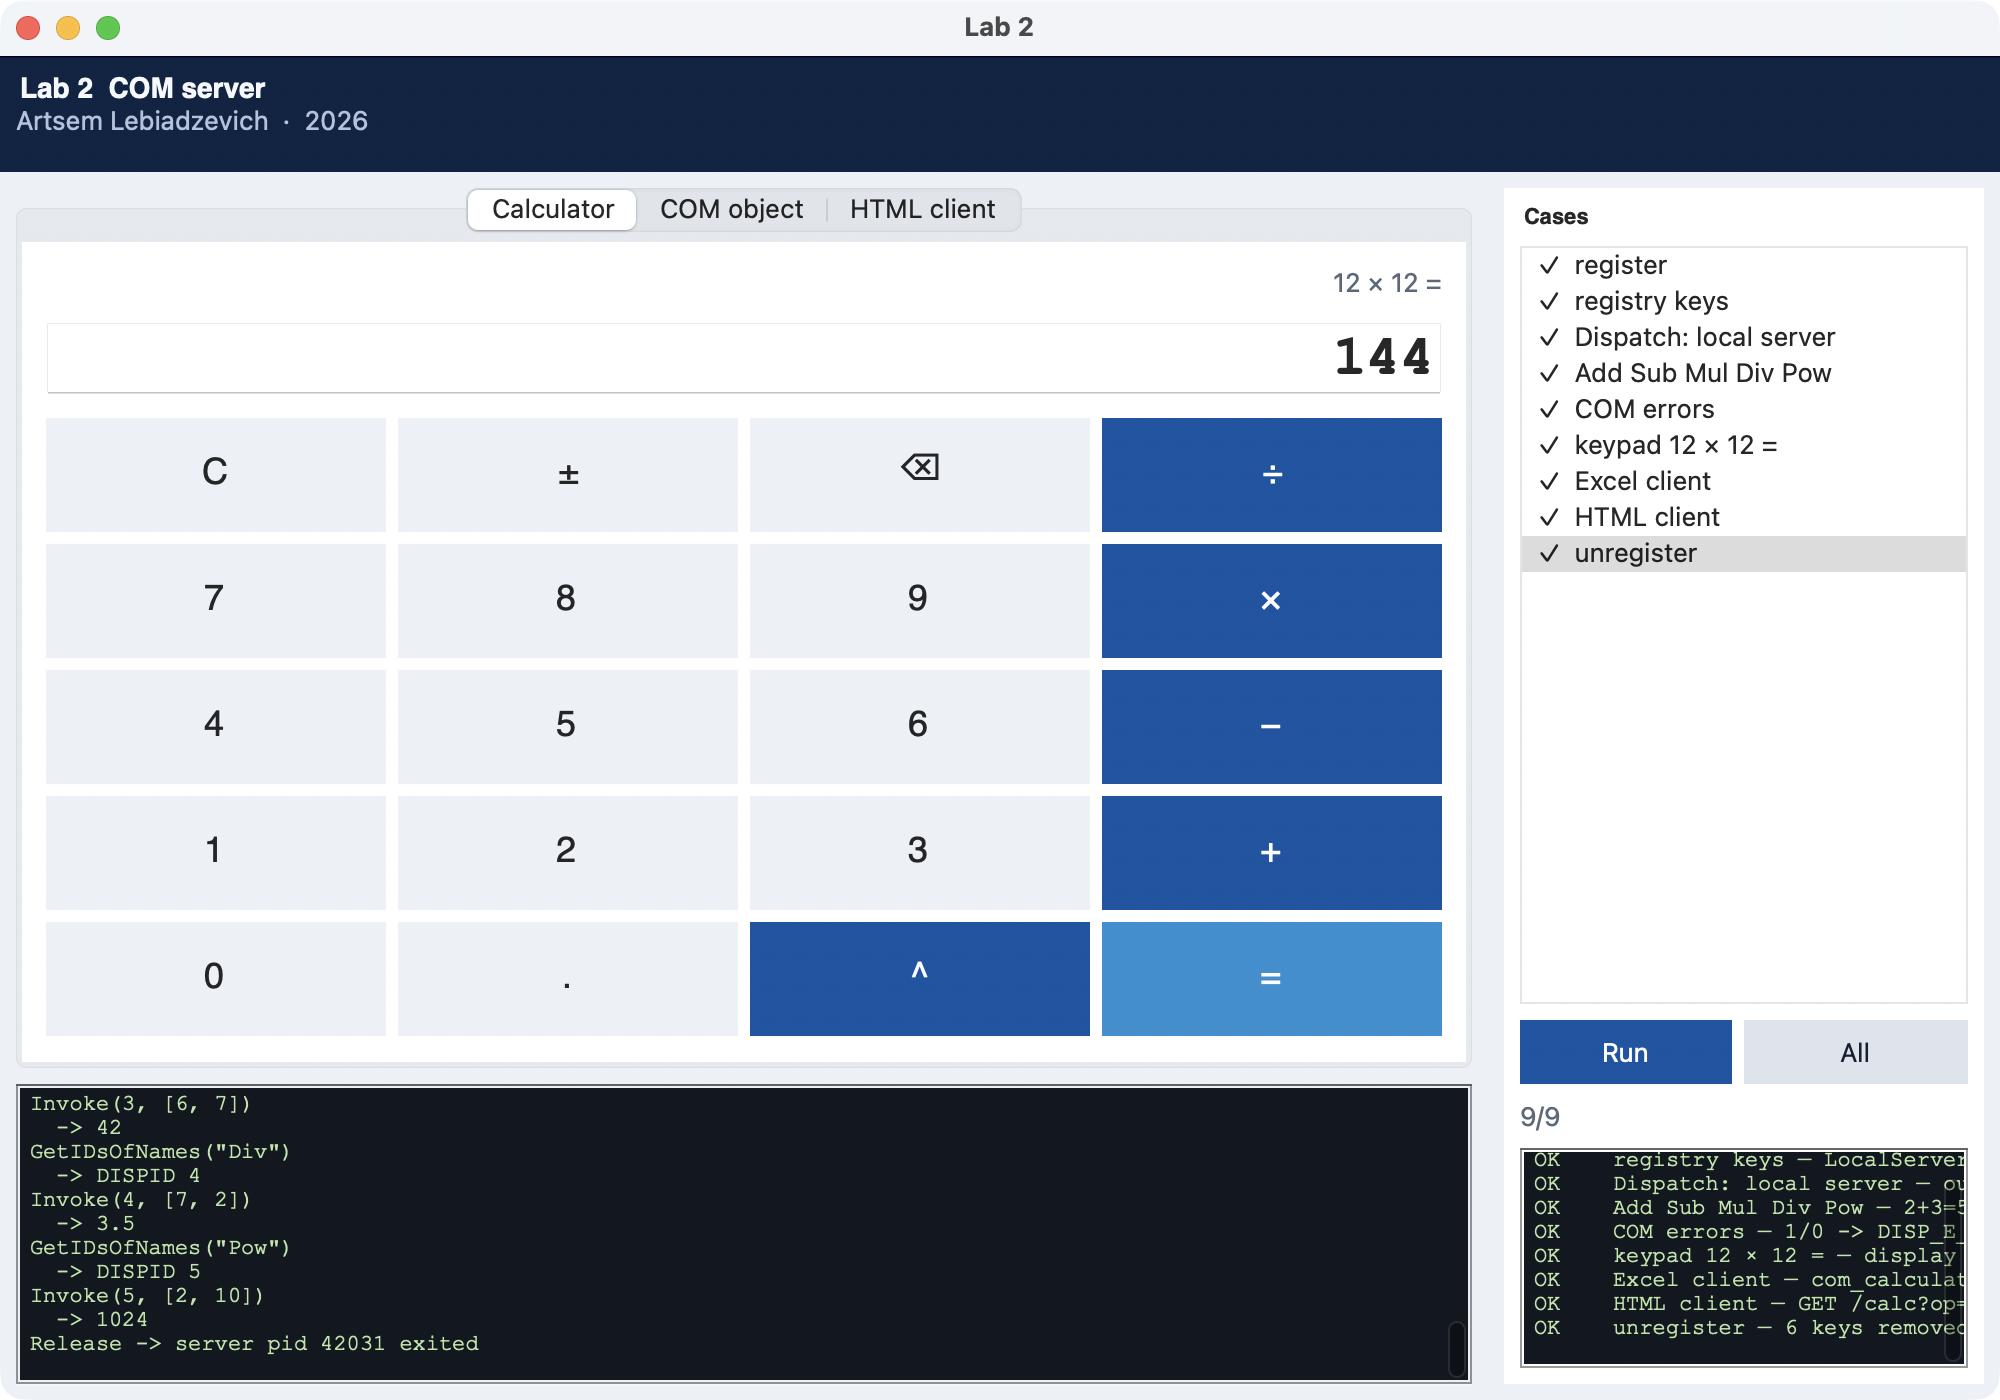
\includegraphics[width=0.95\textwidth]{../screenshots/lab2.png}
\caption{Калькулятор, каждая операция которого выполняется COM-объектом}
\label{fig:calc}
\end{figure}

Деление на ноль (рисунок~\ref{fig:error}) приводит к исключению в процессе сервера.
Клиент получает его в виде кода \texttt{DISP\_E\_EXCEPTION} с текстовым описанием.

\begin{figure}[H]
\centering
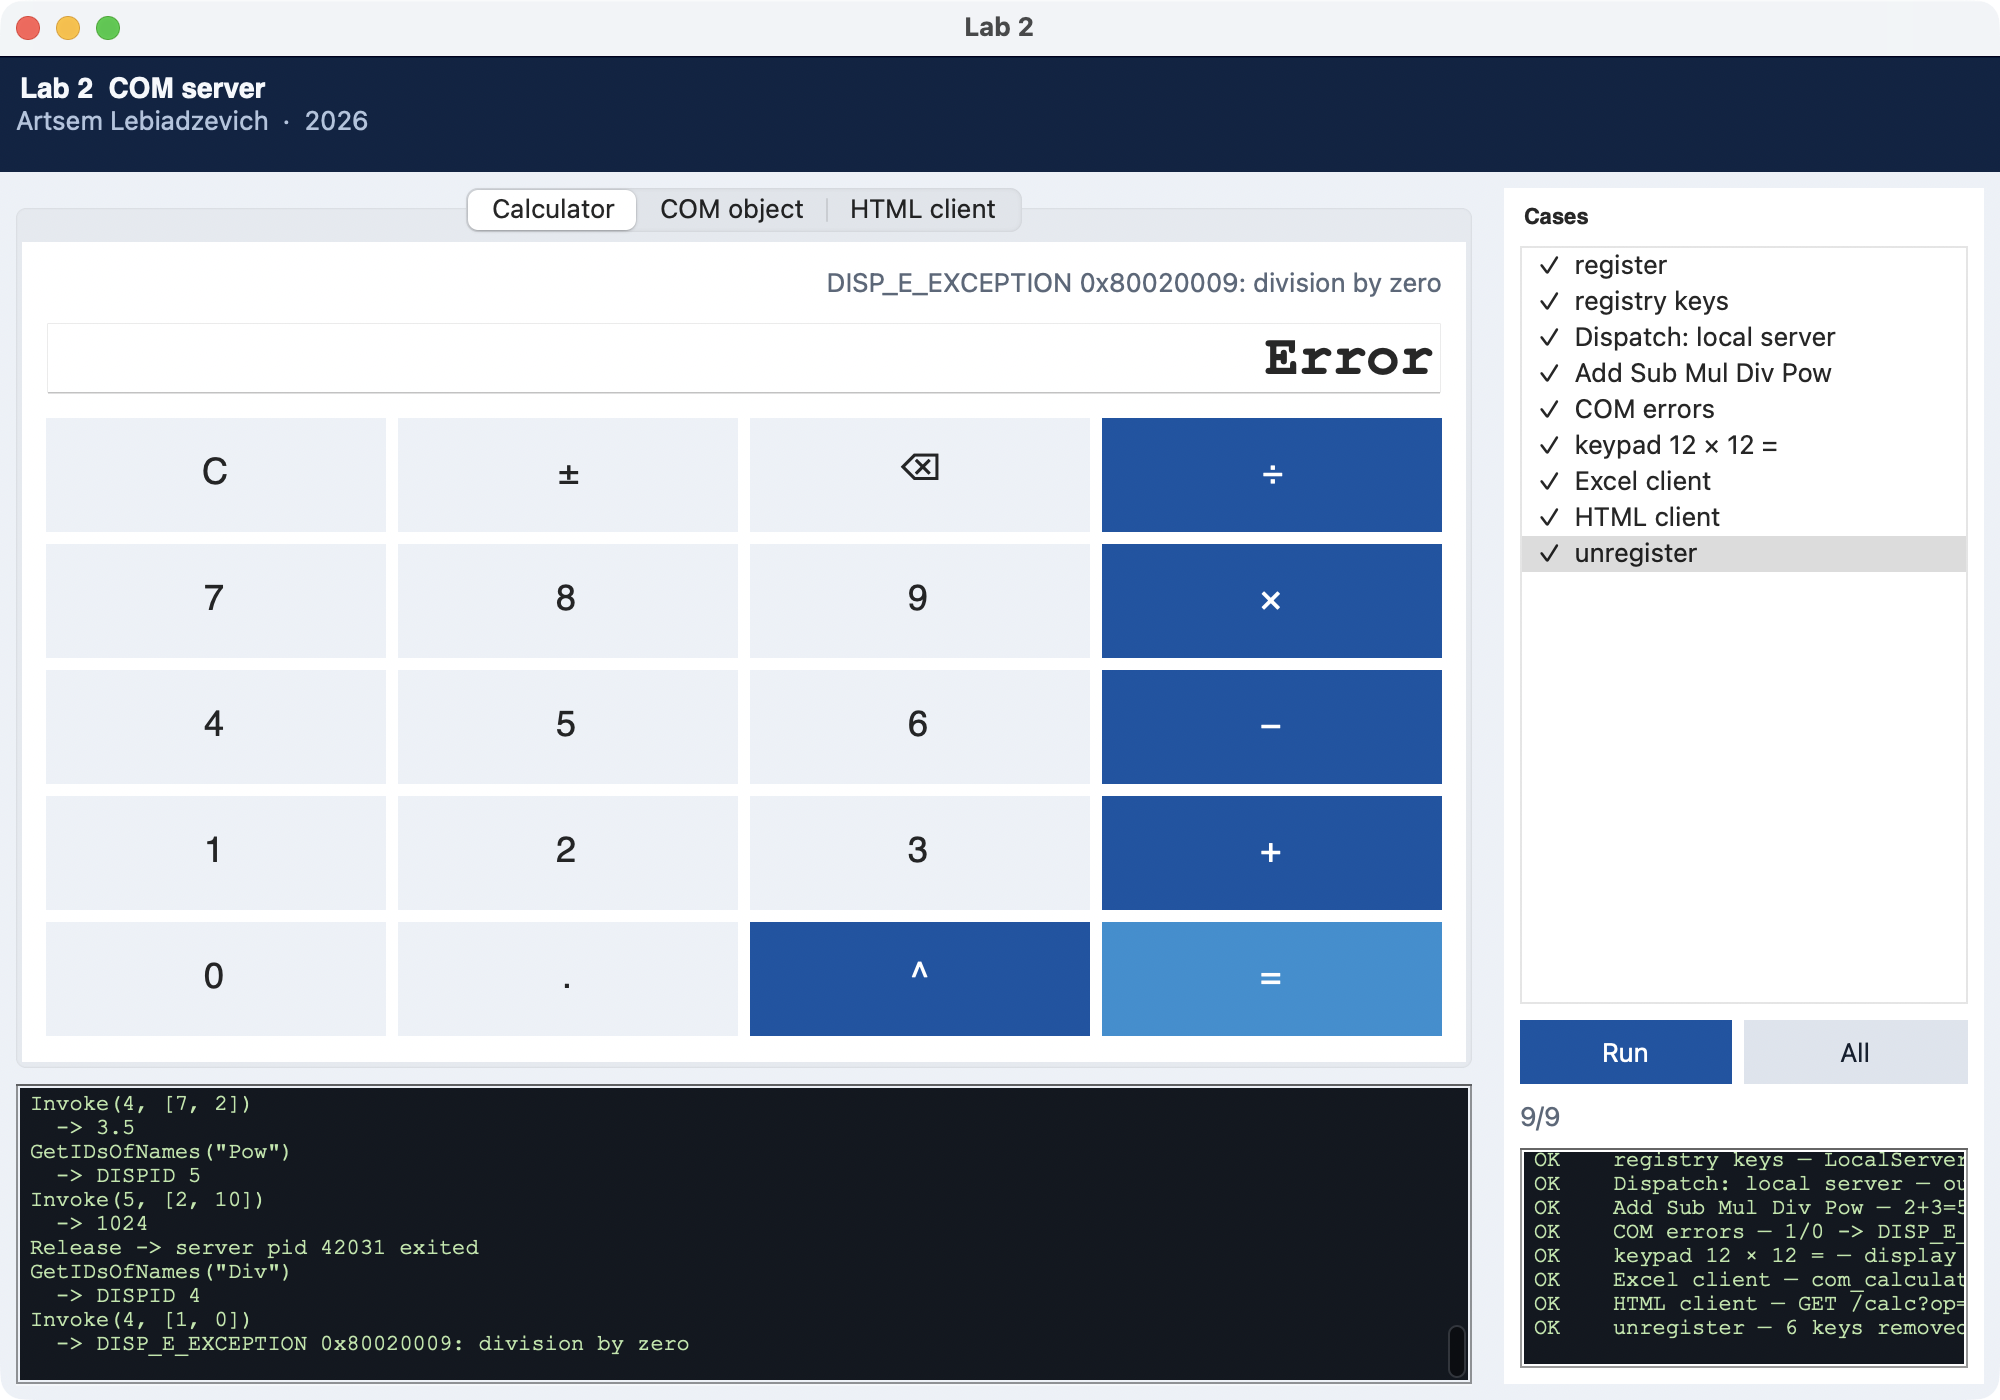
\includegraphics[width=0.95\textwidth]{../screenshots/lab2_error.png}
\caption{Ошибка сервера, переданная клиенту кодом HRESULT}
\label{fig:error}
\end{figure}

На рисунке~\ref{fig:com} показаны ключи реестра после регистрации и состояние объекта:
класс зарегистрирован, сервер работает в отдельном процессе.

\begin{figure}[H]
\centering
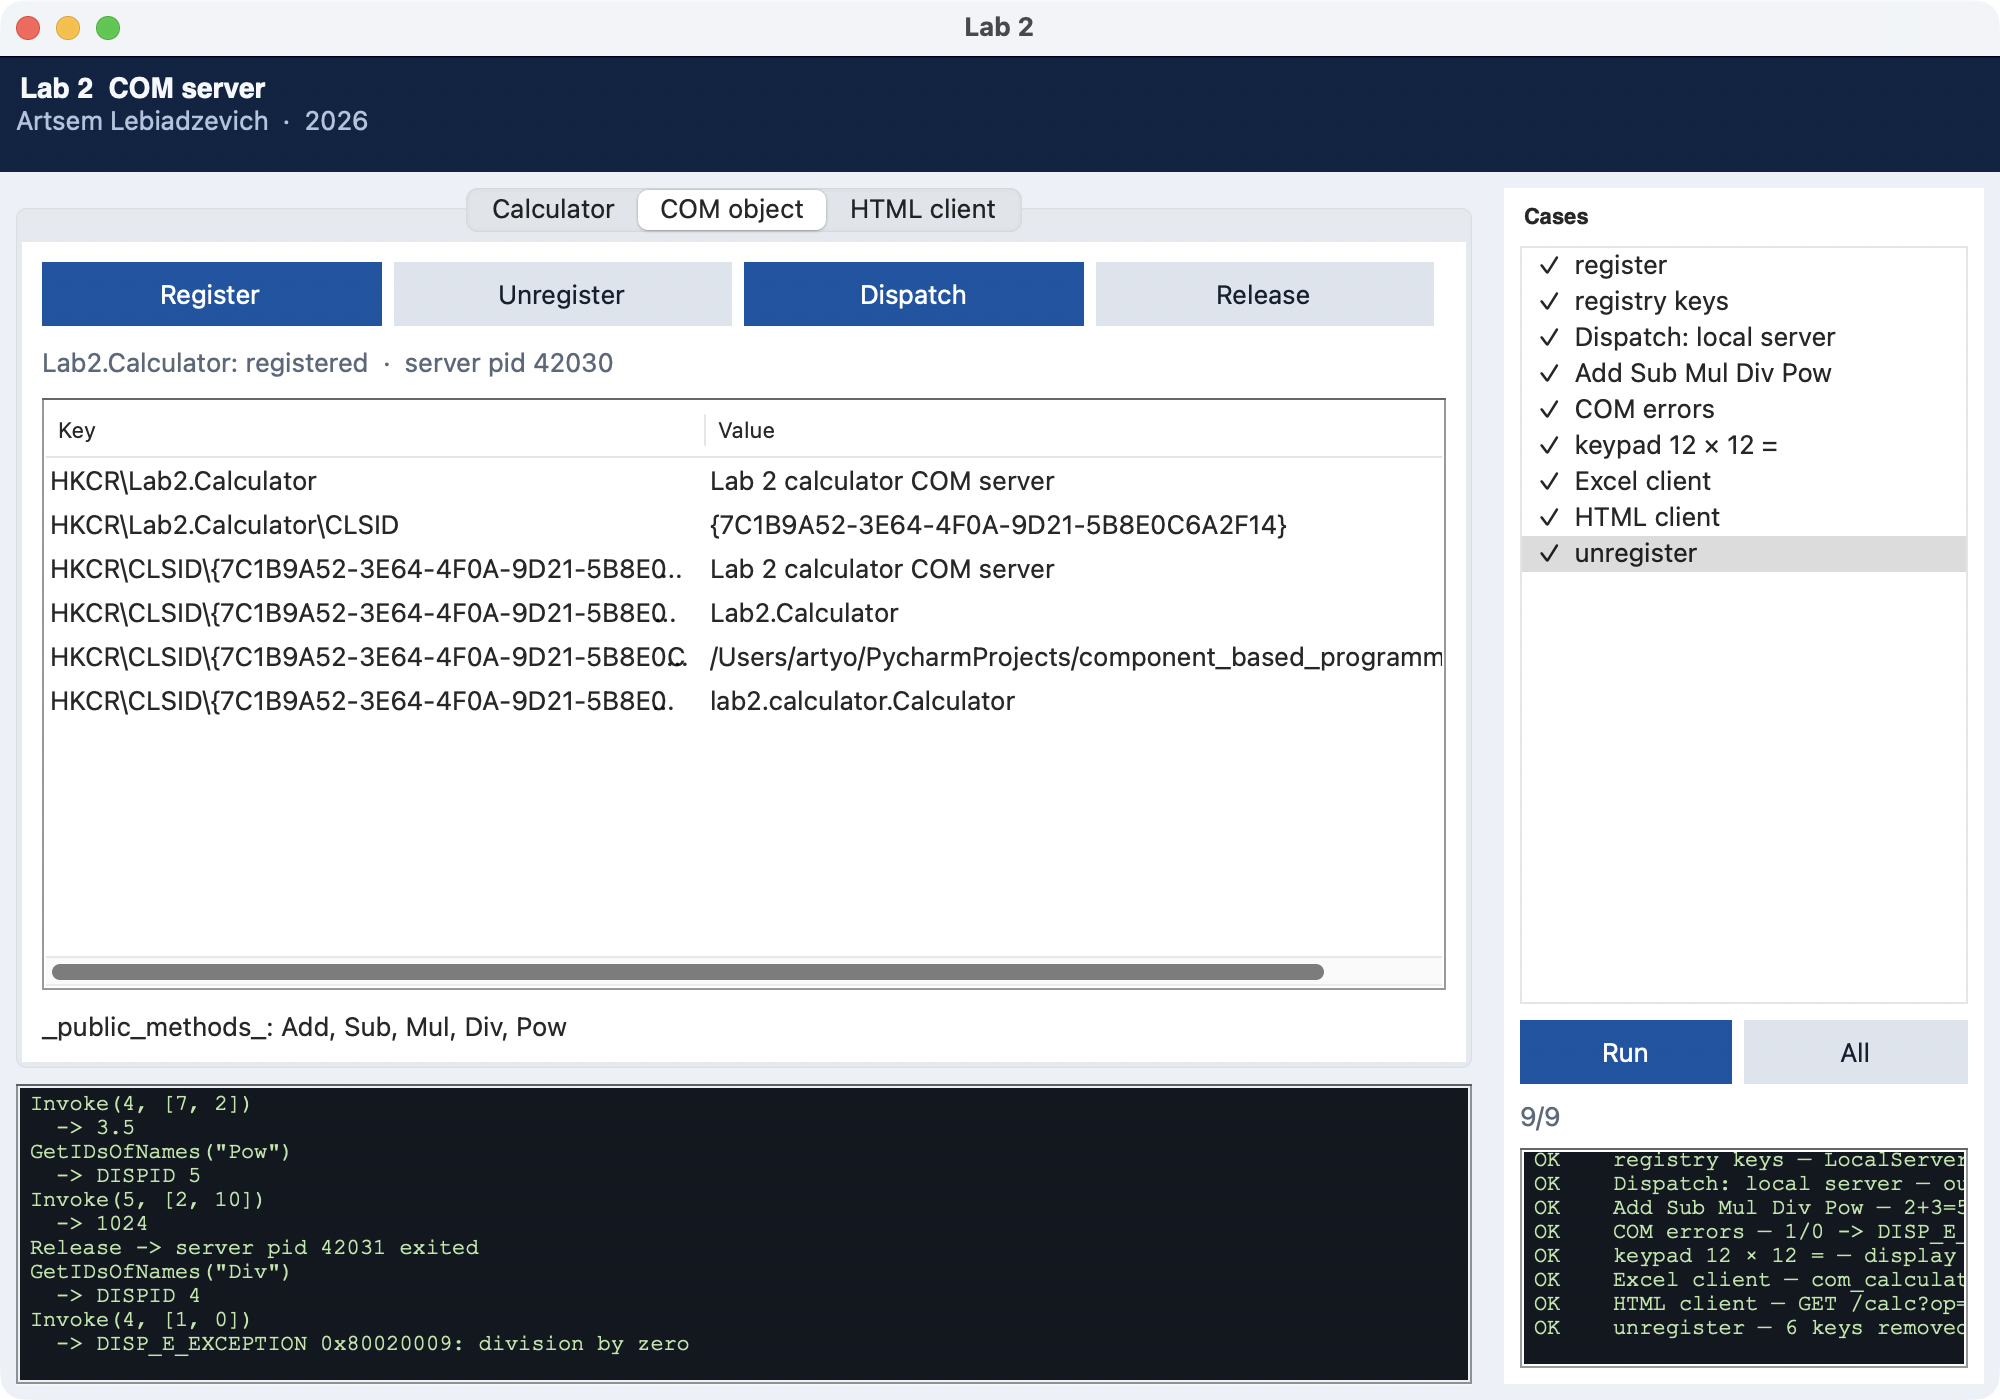
\includegraphics[width=0.95\textwidth]{../screenshots/lab2_com.png}
\caption{Ключи реестра и управление жизненным циклом объекта}
\label{fig:com}
\end{figure}

HTML-клиент (рисунок~\ref{fig:html}) вычисляет $2^{10}$ через тот же COM-объект и
выводит имя и идентификатор класса.

\begin{figure}[H]
\centering
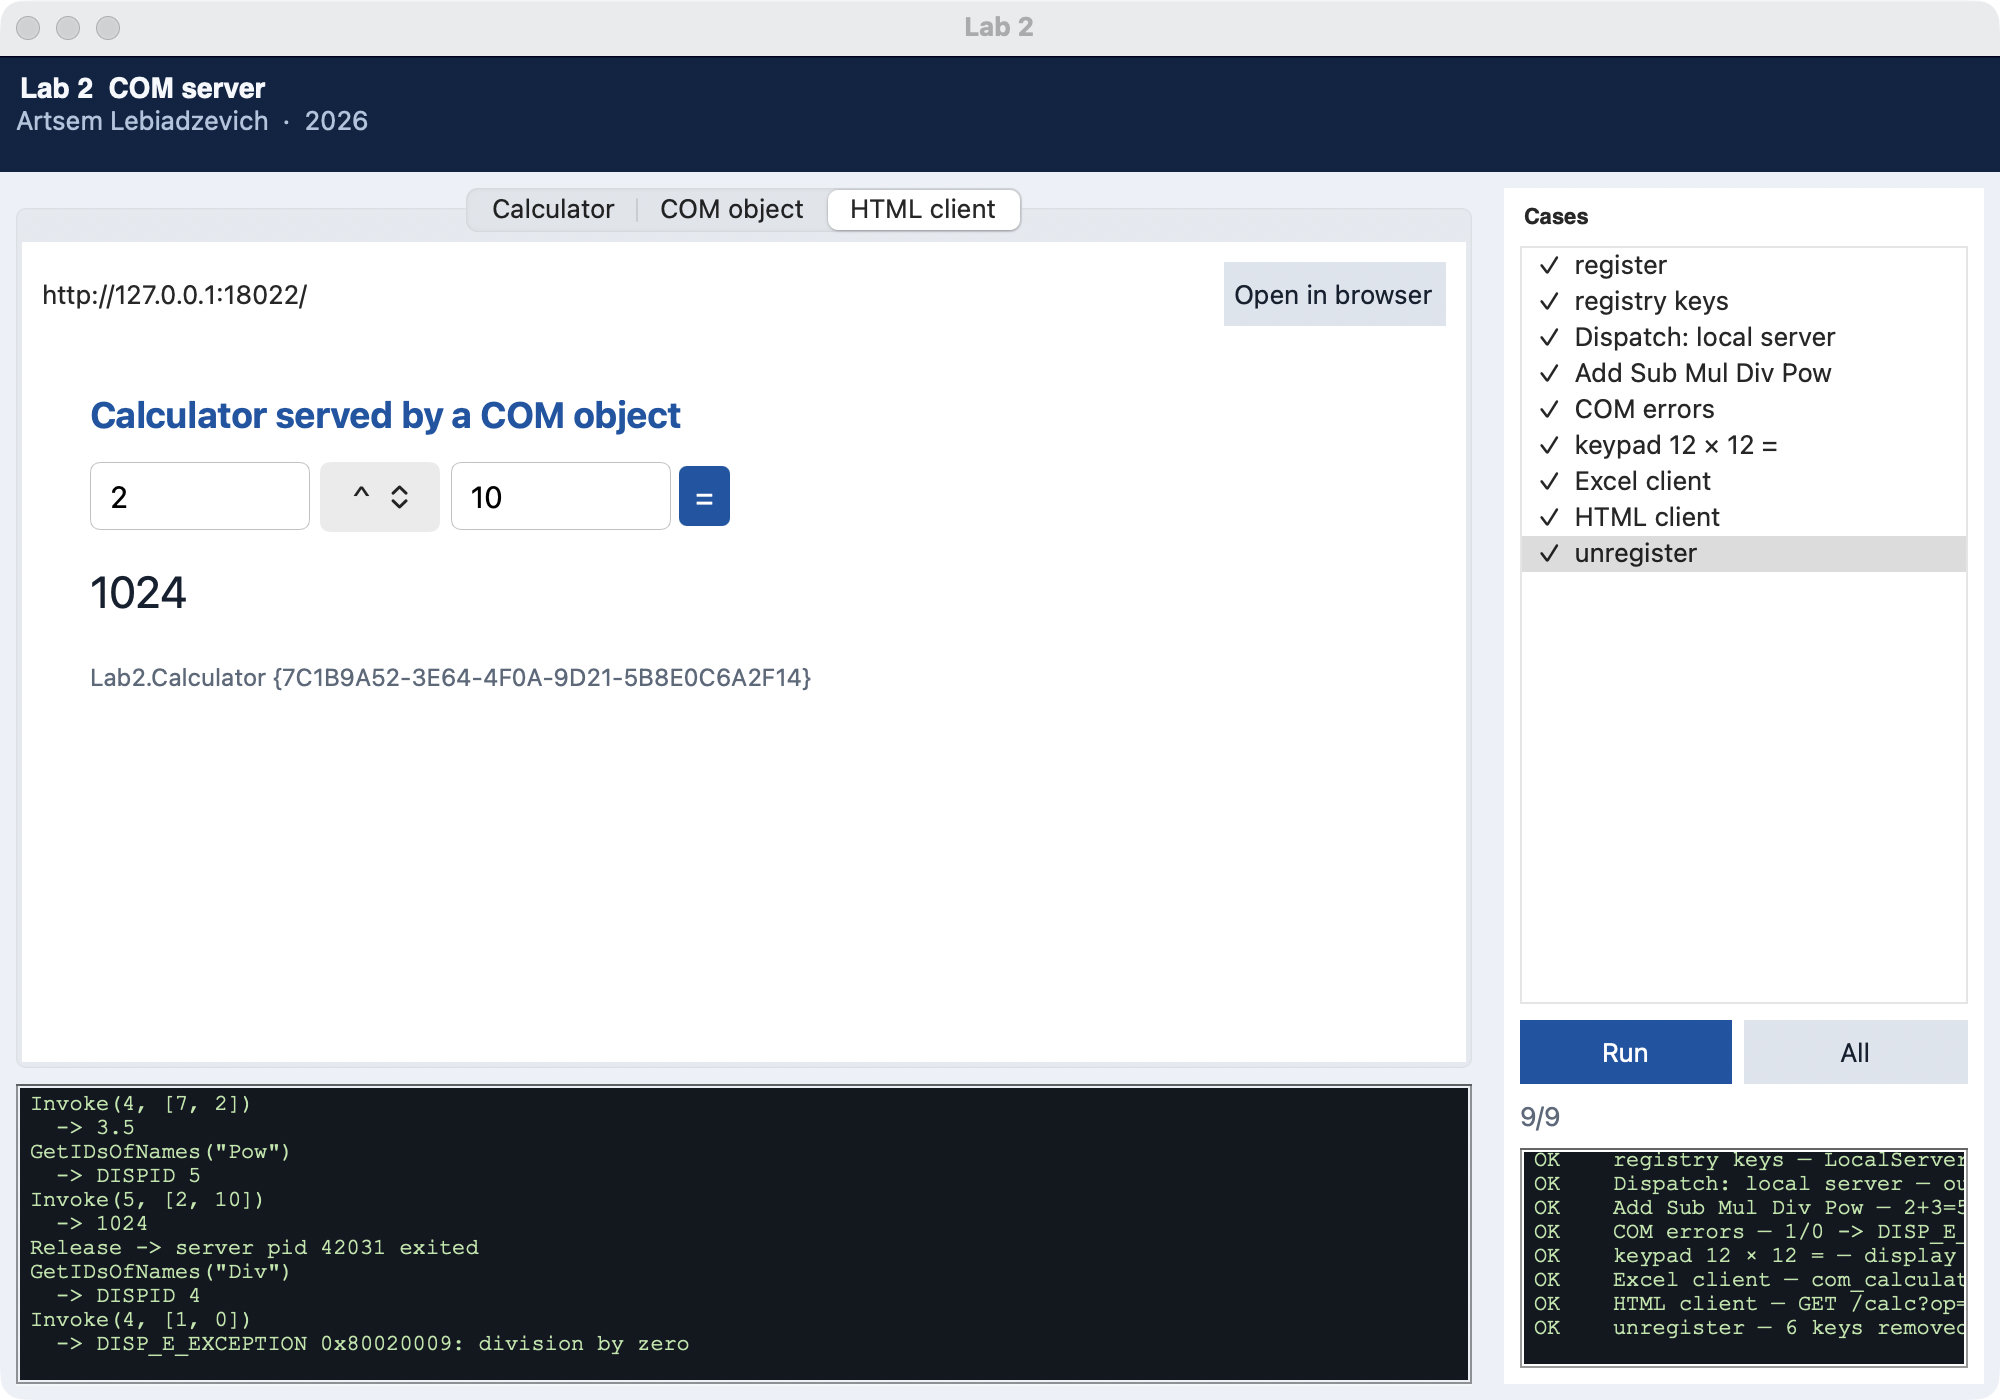
\includegraphics[width=0.95\textwidth]{../screenshots/lab2_html.png}
\caption{HTML-страница, работающая с COM-объектом через серверное приложение}
\label{fig:html}
\end{figure}

Команда \texttt{python main.py -{}-lab 2} выполняет те же сценарии без окна. Её вывод
приведён в листинге~\ref{lst:cli}: сначала ключи реестра, затем журнал вызовов и итоги
сценариев.

\lstinputlisting[style=plain, caption={Вывод программы}, label={lst:cli}]{listings/cli_output.txt}

Сводка по сценариям приведена в таблице~\ref{tab:results}.

\begin{table}[H]
\caption{Проверяемые сценарии}
\label{tab:results}
\centering
\begin{tabularx}{\textwidth}{lLl}
\toprule
Сценарий & Что проверяется & Итог \\
\midrule
register & ProgID указывает на CLSID & да \\
registry keys & CLSID указывает на команду запуска и обратно на ProgID & да \\
Dispatch & сервер работает в другом процессе & да \\
Add Sub Mul Div Pow & пять операций дают 5, $-3$, 42, 3{,}5 и 1024 & да \\
COM errors & деление на ноль и скрытый метод дают коды ошибок & да \\
keypad & нажатия клавиш $12 \times 12 =$ дают 144 & да \\
Excel client & таблица заполнена результатами объекта & да \\
HTML client & запрос \texttt{/calc} возвращает 1024 & да \\
unregister & после отмены регистрации \texttt{Dispatch} даёт
\texttt{CO\_E\_CLASSSTRING} & да \\
\bottomrule
\end{tabularx}
\end{table}

Кроме сценариев окна, написаны автоматические тесты: они проверяют, что сервер
выполняется в другом процессе, пять операций, три кода ошибок и ответ HTML-клиента.
Все тесты проходят.

\section{Ответы на контрольные вопросы}

\textbf{1. Что такое COM-сервер и для чего он используется?} COM-сервер --- программный
компонент, который предоставляет объекты через интерфейсы COM, так что к ним могут
обращаться программы на других языках и из других процессов. Применяется для
автоматизации приложений Office, межпроцессного взаимодействия и повторного
использования существующих компонентов.

\textbf{2. Что такое параметр CLSID и как его создать?} CLSID --- 128-битный
идентификатор COM-класса (GUID). Создаётся один раз, например функцией
\texttt{uuid.uuid4()}, утилитой \texttt{guidgen} или функцией
\texttt{pythoncom.CreateGuid()}, и после этого не меняется.

\textbf{3. В каком разделе реестра находится CLSID?} В разделе
\texttt{HKEY\_CLASSES\_ROOT\textbackslash CLSID}. Этот раздел является объединённым
представлением ветвей \texttt{Software\textbackslash Classes} из
\texttt{HKEY\_LOCAL\_MACHINE} и \texttt{HKEY\_CURRENT\_USER}. На идентификатор
указывает ключ \texttt{HKEY\_CLASSES\_ROOT\textbackslash <ProgID>\textbackslash CLSID}.

\textbf{4. Как интегрировать COM-сервер в веб-приложение?} Браузер создавать
COM-объекты не может, поэтому используется серверное приложение (Flask или встроенный
HTTP-сервер): оно создаёт объект функцией \texttt{Dispatch}, вызывает его метод и
возвращает результат странице в виде HTML или JSON.

\sectioncenter{Заключение}

В ходе лабораторной работы изучена компонентная объектная модель COM и создан
COM-сервер на языке Python, выполняющий сложение, вычитание, умножение, деление и
возведение в степень. Сервер используется тремя клиентами: графическим калькулятором,
таблицей Excel и HTML-страницей, причём ни один из них не импортирует код
калькулятора --- все обращаются к объекту по имени \texttt{Lab2.Calculator}.

Главный практический вывод состоит в том, что клиент компонента знает только имя, а
связь имени с кодом хранит система. Поэтому регистрация является обязательным
отдельным шагом: при отсутствии записи в реестре исправный и доступный код сервера
клиенту недоступен, и активация завершается ошибкой \texttt{CO\_E\_CLASSSTRING}.

Сравнение систем показало, что компонентный подход не ограничен Windows. В Linux
вызовы между процессами и активацию по требованию обеспечивает шина D-Bus, в macOS ---
XPC и Apple Events, а роль реестра выполняют каталоги с файлами описаний. Отличие
Windows в том, что эти возможности объединены в одну модель с единым реестром. Сами
COM-объекты между системами не переносятся, поэтому на macOS работа выполнена на
переносимой модели COM, а вариант с библиотекой \texttt{pywin32} и макросом VBA
подготовлен для запуска в Windows.

\sectioncenter{Список использованных источников}

\begin{enumerate}
\item Герман, О.~В. COM-сервера: лекция и лабораторная работа по дисциплине
<<Технологии компонентного программирования>> / О.~В.~Герман. --- Минск: БГУИР, 2024.
\item Роджерсон, Д. Основы COM / Д.~Роджерсон. --- М.: Русская редакция, 2000. ---
400~с.
\item Бокс, Д. Сущность технологии COM / Д.~Бокс. --- СПб.: Питер, 2001. --- 400~с.
\item Szyperski, C. Component Software: Beyond Object-Oriented Programming /
C.~Szyperski. --- 2nd ed. --- Boston: Addison-Wesley, 2002. --- 624~p.
\item Hammond, M. Python Programming on Win32 / M.~Hammond, A.~Robinson. ---
Sebastopol: O'Reilly, 2000. --- 652~p.
\item D-Bus Specification [Электронный ресурс]. --- Режим доступа:
\url{https://dbus.freedesktop.org/doc/dbus-specification.html}.
\end{enumerate}

\end{document}
